\documentclass{article}
\usepackage{aligned-overset}
\usepackage{amsmath}
\usepackage{amssymb}
\usepackage{bm}
\usepackage[shortlabels]{enumitem}
\usepackage{hyperref}
\usepackage[utf8]{inputenc}
\usepackage{mathtools}
\usepackage{physics}
\usepackage{tabularx}
\usepackage{titling}
\usepackage{fancyhdr}
\usepackage{xfrac}
\usepackage{pgfplots}

\pgfplotsset{compat = newest}
\usetikzlibrary{intersections}
\usepgfplotslibrary{fillbetween}


\author{}
\date{SoSe 2021}
\title{Hausaufgabe 02 Analysis - Weiterführende Konzepte}

\pagestyle{fancy}
\fancyhf{}
\lhead{\thetitle}
\rhead{\theauthor}
\lfoot{\thedate}
\rfoot{Seite \thepage}

\begin{document}

\section*{Hausaufgabe 1}

Untersuchen Sie, ob die folgenden Aussagen wahr oder falsch sind.
Begründen Sie Ihre Antworten.

\begin{enumerate}[(i)]
\item Die Funktion $F(x) \coloneqq x\abs{x}, x \in [-1,1]$, ist die Stammfunktion einer
  Funktion $f \in R([-1, 1])$.

  \label{dia:1.1}
  \begin{tikzpicture}
    \begin{axis}[
        axis lines=middle,
        xmax = 1.2,
        xmin = -1.2,
        ymax = 1.2,
        ymin = -1.2,]
      \addplot [
        domain=-1:1,
        name path=f,
        samples=100,
        very thick, blue]{x * abs(x)};
    \end{axis}
  \end{tikzpicture}

  $F(x) = \begin{cases}
    x^2 & x \geq 0 \\
    - x^2 & x < 0 \\
  \end{cases}, F'(x) = \begin{cases}
    2x & x \geq 0 \\
    -2x & x < 0 \\
  \end{cases} = 2 \abs{x} = f(x)$.
  Die Funktion $f(x)$ ist auf dem kompakten Intervall $[-1, 1]$ stetig, somit ist
  $f \in R([-1, 1])$ und die Aussage ist wahr.
  
\item Die Funktion $f(x) \coloneqq \text{sign}(x) \sqrt{\abs{x}}, x \in [-1,1]$, besitzt
  auf $[-1,1]$ eine Stammfunktion.

  \label{dia:1.2}
  \begin{tikzpicture}
    \begin{axis}[
      axis lines=middle,
      xmax = 1.2,
      xmin = -1.2,
      ymax = 1.2,
      ymin = -1.2,]
      \addplot [
        domain=-1:1,
        name path=f,
        samples=100,
        very thick, blue]{sign(x) * sqrt(abs(x))};
    \end{axis}
  \end{tikzpicture}

  Die Funktion ist auf den Intervallen $[-1, 0)$ und $(0, 1]$ stetig.
  Weiterhin ist $\lim_{x \to 0-} f(x) = \lim_{x \to 0+} f(x) = f(x) = 0$.
  Somit ist die Funktion auf dem kompakten Intervall $[-1, 1]$ stetig und
  besitzt auf diesem Intervall eine Stammfunktion.
  Damit ist die Aussage wahr.
  
\item Die Funktion $f(x) \coloneqq \text{sign}(x) \sqrt{\abs{x + \frac{1}{2}}}, x \in [-1,1]$, besitzt
  auf $[-1,1]$ eine Stammfunktion.

  \label{dia:1.2}
  \begin{tikzpicture}
    \begin{axis}[
        axis lines=middle,
        xmax = 1.2,
        xmin = -1.2,
        ymax = 1.2,
        ymin = -1.2,]
      \addplot [
        domain=-1:-0.01,
        name path=f,
        samples=100,
        very thick, blue]{sign(x) * sqrt(abs(x + 0.5))};
      \node [
        circle,
        fill,
        inner sep=1pt, blue] at (0,0) {};
      \addplot [
        domain=0.01:1,
        name path=f,
        samples=100,
        very thick, blue]{sign(x) * sqrt(abs(x + 0.5))};
    \end{axis}
  \end{tikzpicture}

  $\lim_{x \to 0-} f(x) = - \sqrt{\frac{1}{2}}, \lim_{x \to 0+} f(x) = \sqrt{\frac{1}{2}}$ und $f(0) = 0$.
  Damit besitzt die Funktion an der Stelle $0$ einen Sprung.
  Aus dem Satz von Darboux folgt, dass die Funktion auf dem Intervall $[-1, 1]$ keine Stammfunktion besitzt.
\end{enumerate}

\section*{Hausaufgabe 2}

\section*{Hausaufgabe 3}

\newpage
\section*{Hausaufgabe 4}

Die Funktionen $f, g \colon \mathbb{R} \to \mathbb{R}$ definiert durch
$f(x) = x^3 - 2x^2 + x$ und $g(x) = \frac{1}{2}x^2$ umschließen im 1.
Quadranten einen beschränkten Berebich $B$.
Skizzieren Sie diesen Bereich $B$ und berechnen Sie dessen Flächeninhalt.
\\

\label{dia:4}
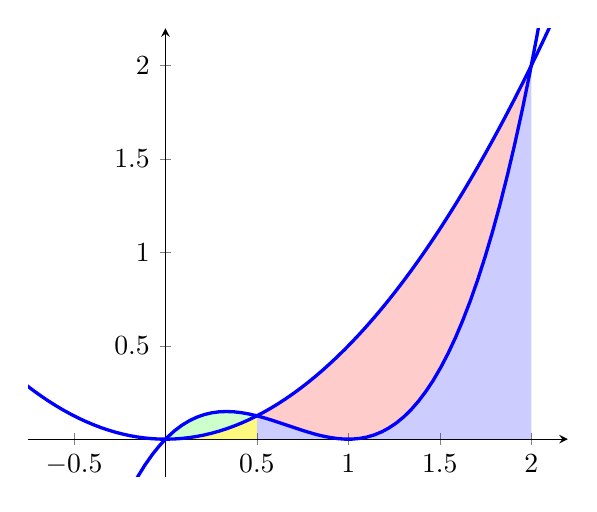
\begin{tikzpicture}
  \begin{axis}[
      axis lines=middle,
      xmax = 2.2,
      xmin = -0.75,
      ymax = 2.2,
      ymin = -0.2,]
    \addplot [
      domain=-1:3,
      name path=f,
      samples=100,
      very thick, blue]{x^3 - 2*x^2 + x};
    \path[name path=axisa] (axis cs:0,0) -- (axis cs:0.5,0);
    \path[name path=axisb] (axis cs:0.5,0) -- (axis cs:2,0);
    \addplot [
      thick,
      color=blue,
      fill=blue, 
      fill opacity=0.2
    ]
    fill between[
      of=f and axisb,
      soft clip={domain=0.5:2},
    ];
    \addplot [
      domain=-1:3,
      name path=g,
      samples=100,
      very thick, blue]{0.5 * x^2};
    \addplot [
      thick,
      color=yellow,
      fill=yellow, 
      fill opacity=0.5
    ]
    fill between[
      of=g and axisa,
      soft clip={domain=0:0.5},
    ];
    \addplot [
      thick,
      color=green,
      fill=green, 
      fill opacity=0.2
    ]
    fill between[
      of=f and g,
      soft clip={domain=0:0.5},
    ];
    \addplot [
      thick,
      color=red,
      fill=red, 
      fill opacity=0.2
    ]
    fill between[
      of=f and g,
      soft clip={domain=0.5:2},
    ];  
  \end{axis}
\end{tikzpicture}

\textbf{Schnittstellen der beiden Funktionen berechnen}:
\begin{align*}
  f(x) &= g(x) \\
  x^3 - 2x^2 + x &= \frac{1}{2}x^2 && | :x \text{ $x_1 = 0$ ist eine Lösung} \\
  x^2 - 2x + 1 &= \frac{1}{2}x && | \cdot 2 \\
  2 x^2 - 4x + 2 &= x && | - x \\
  2 x^2 - 5x + 2 &= 0 \\
\end{align*}

\begin{align*}
  x_{2|3} &= \frac{5 \pm \sqrt{5^2 - 4 \cdot 2 \cdot 2}}{2 \cdot 2} \\
          &= \frac{5 \pm \sqrt{9}}{4} \\
  x_2 &= 0.5, \, x_3 = 2 
\end{align*}

\textbf{Stammfunktionen von $g$ und $f$ ermitteln}
\begin{align*}
  F(x) &= \frac{1}{4}x^4 - \frac{2}{3}x^3 + \frac{1}{2}x^2 \\
  G(x) &= \frac{1}{6}x^3 
\end{align*}

\newpage
\textbf{Fläche B berechnen}:

Die Fläche B setzt sich aus zwei Teilflächen - im \hyperref[dia:4]{Diagramm}
grün und rot markiert - zusammen.
Der Inhalt der grünen Teilfläche ($B_1$) errechnet sich aus
$B_1 = \int_{x_1}^{x_2} f(x) dx - \int_{x_1}^{x_2} g(x) dx$ und der Inhalt der roten
Teilfläche ($B_2$) aus
$B_2 = \int_{x_2}^{x_3} g(x) dx - \int_{x_2}^{x_3} f(x) dx$
\begin{align*}
  B_1 &= \left( F(x_2) - F(x_1) \right) - \left( G(x_2) - G(x_1) \right) \\
      &= F(x_2) - F(x_1) - G(x_2) + G(x_1) \\
      &= \sfrac{1}{4}(x_2)^4 - \sfrac{2}{3}(x_2)^3 + \sfrac{1}{2}(x_2)^2 - \sfrac{1}{4}(x_1)^4 + \sfrac{2}{3}(x_1)^3 - \sfrac{1}{2}(x_1)^2 -
        \sfrac{1}{6}(x_2)^3 + \sfrac{1}{6}(x_1)^3 \\
      &= \sfrac{1}{4}(x_2)^4 - \sfrac{5}{6}(x_2)^3 + \sfrac{1}{2}(x_2)^2 - \sfrac{1}{4}(x_1)^4 + \sfrac{5}{6}(x_1)^3 - \sfrac{1}{2}(x_1)^2 \\
      &= \sfrac{1}{4}\left(\sfrac{1}{2}\right)^4 - \sfrac{5}{6}\left(\sfrac{1}{2}\right)^3 + \sfrac{1}{2}\left(\sfrac{1}{2}\right)^2 -
        \sfrac{1}{4}(0)^4 + \sfrac{5}{6}(0)^3 - \sfrac{1}{2}(0)^2 \\
      &= \frac{7}{192}
\end{align*}
\begin{align*}
  B_2 &=\left( G(x_3) - G(x_2) \right) - \left( F(x_3) - F(x_2) \right) \\
      &= G(x_3) - G(x_2) - F(x_3) + F(x_2) \\
      &= \sfrac{1}{6}(x_3)^3 - \sfrac{1}{6}(x_2)^3 - \sfrac{1}{4}(x_3)^4 + \sfrac{2}{3}(x_3)^3 - \sfrac{1}{2}(x_3)^2 +
        \sfrac{1}{4}(x_2)^4 - \sfrac{2}{3}(x_2)^3 + \sfrac{1}{2}(x_2)^2 \\
      &= - \sfrac{1}{4}(x_3)^4 + \sfrac{5}{6}(x_3)^3 - \sfrac{1}{2}(x_3)^2 +
        \sfrac{1}{4}(x_2)^4 - \sfrac{5}{6}(x_2)^3 + \sfrac{1}{2}(x_2)^2 \\
      &= - \sfrac{1}{4}(2)^4 + \sfrac{5}{6}(2)^3 - \sfrac{1}{2}(2)^2 + \sfrac{1}{4}\left(\sfrac{1}{2}\right)^4 -
        \sfrac{5}{6}\left(\sfrac{1}{2}\right)^3 + \sfrac{1}{2}\left(\sfrac{1}{2}\right)^2 \\
      &= \frac{45}{64}
\end{align*}

$B = B_1 + B_2 = \frac{7}{192} + \frac{45}{64} = \frac{142}{192}$

\end{document}